\documentclass[conference]{hehe}
\usepackage[utf8]{inputenc}
\IEEEoverridecommandlockouts

\usepackage{cite}
\usepackage{amsmath,amssymb,amsfonts}
\usepackage{algorithmic}
\usepackage{graphicx}
\usepackage{amsthm}
\usepackage{textcomp}
\usepackage{xcolor}
\usepackage{float}
\def\BibTeX{{\rm B\kern-.05em{\sc i\kern-.025em b}\kern-.08em
    T\kern-.1667em\lower.7ex\hbox{E}\kern-.125emX}}
\newtheorem{definition}{Definition}
\begin{document}

\title{Review on Games, norms and obligations
\\
{\footnotesize \textsuperscript{}}
\thanks{}
}

\author{\IEEEauthorblockN{Josua Potschien}
\IEEEauthorblockA{\textit{696346} \\
\textit{}}
\and
\IEEEauthorblockN{Chris Venn}
\IEEEauthorblockA{\textit{676120} \\
\textit{}}

}

\maketitle

\begin{abstract}
This review will give you a short overview about the development of norms, normative systems, the problems with the traditional approaches and most importantly about the approach of violation games. We will talk about the idea of violation games as well as the advantages and disadvantages for practical use.
\end{abstract}

\begin{IEEEkeywords}
norms, normative systems, autonomous systems, violation games
\end{IEEEkeywords}



\section{What is a norm?}

First, we talk about the meaning of a norm. We just keep the standardized definition of a social norm we all know. It can be thought of as: "rules that prescribe what people should and should not do given their social surroundings"\cite{b1}. For example it is wrong to cheat on your significant other, it is good to finish something in time and it's bad to hijack a plane.
\subsection{Definition of normative systems}
Van der Torre gives us the first definition of a normative system based on good and bad.\\

\begin{definition}
A normative system is a description of good and
bad. \cite{b2}
\end{definition}

It is a popular way to look at normative reasoning, but often it is insufficient. Imagine the following. A plane full of passengers got hijacked and the terrorists threaten to crash it into a skyscraper. Now you have a moral dilemma.\\
A: You can shoot down the plane and you prevent higher casualties.\\
B: When you don't shoot down the plane innocent people will die.

Therefore many definitions for a normative system have been proposed and each one has its own loopholes.


\begin{definition}
A normative system is a description
of violation conditions. \cite{b2}\\
\end{definition}

In terms of our hijacked-plane-example we can now say that hijacking a plane is a violation followed by sanctions for this action.\\
But also the sanctions that will follow for hijacking a plane are not very clear. For example what is an adequate sanction or is it even possible to execute the sanction in case of hijacking a plane?\\
Despite the violation of the norm there can't be any sanctions for this violation because the terrorist dies when crashing the plane and he now can't be sanctioned anymore.\\

\begin{definition}
A normative system is a set of rules used to guide,
control, or regulate desired system behavior.\cite{b2}\\
\end{definition}

This definition also has its flaws. If you consider a traffic problem in a large city you can create new norms to change peoples behavior. For example if you create a norm where you have to use a bike for short distances and a car for long distances. This norm can easily be violated because in practice it is hard to check if it was necessary to use the car for a certain purpose.\\
Even though this is a good definition to guide systems behavior it is still not the best solution because of the explained side effects.

In conclusion we can say that none of the above definitions are perfect and therefore you may look for a better alternative to define a normative system.

\subsection{What is an autonomous system?}
We shall have an idea of an autonomous system later so we shortly sum up the most important aspects.\\

A strongly autonomous system can create and enforce its own laws/norms. It is a set of independent system and each system can make its own local norms but still must be regulated by global norms within the system (e.g the EU and its countries).\\
At best there are some monitor systems that can sanction violators of the system to check if the global norms are in force.\\


\section{Problems with the traditional approach}
You have to consider different areas for the usage of deontic logic. The traditional approach refers to the concepts of deontic logic which have been worked out over the past decades.  Van der Torre explains the problems that will arise in some of those areas.\\
%\textbf{Philosophers} criticize that norms direct behavior rather than describing it and they are neither true or false. \\
\textbf{Lawyers} have similar problems with the traditional approach of deontic logic. The argumentation in law is based on conflicts but deontic logic does not include a theory of conflict resolution. Another reason is that most legal reasoning problems are classification problems concerned with legal ontology, whether a particular case counts as a case for a norm. Lawyers mostly argue how norms must be interpreted. \cite{b2}

\textbf{Computer Scientists}
An important aspect is the specify the behavior if something illegal occures. For example one important problem is when you read and write into a bank account at the same time. So these errors that can occure have to be included in the specification.\\
But with those specifications we have the following problems:\\
- When is a norm redundant?\\
- How to change/merge normative systems?\\
Deontic logic couldn't interpret norms as they were used in some programming languages.\\

Furthermore van der Torre considers on how deontic logic can be based on norm and detachment. Detachment first introduced by David Makinson might be a new deontic logic approach where the traditional model approach fails. At first van der Torre defined the term detachment according to normative systems as follows.\\
\begin{definition}[\textbf{Detachment}]
A normative system is a set of rules together with
a way to detach obligations, permissions and institutional facts in specific situations. \cite{b2}
\end{definition}

Now we can look at an example. So imagine you have a normative system which a rule that said it is forbidden to kill. Or in a logical term: $O(\lnot kill)$.\\
But even if one ever kills he must kill gently\\
($kill \to O(killgently)$).\\
That implies if one person kills another that $killgently \to kill$ holds so killing gently implies to kill.\\
So in other words if you are going to kill someone then you should do it.\\
To solve this paradox you can use the approach of detachment to detach obligations.\\
Let us denote $O(Q | P)$ as $Q$ ought to be the case given $P$.\\
The mistake in the example above was to say that: concluding $O(Q)$ from $O(Q | P)$ and $P$.\\
The proper rule you can now derive from detachment is to only conclude $O(Q)$ from $O(Q | P)$ and $O(P)$.\\

So after the problem with the traditional approach was discussed you also have an idea of how deontic login can be based on norm and detachment.\\
With this thoughts you may now ask if it's possible to combine this approach with with a more complex approach? In the following section van der Torre will introduce the new approach of decision and game theory trying to model complex problems and finally discuss the question of how deontic logic can be based on both, norm and detachment.

\section{Violation games}
In this section we will summarize van der Torres explanation of a newer approach trying to combine the definitions of normative systems and the different areas of deontic logic. A violation game is defined by norms which act as rules. So after norms have been created you can play violation games within this normative system. It is a more complex way to analyze a situation and define violation.\\
To understand the idea of a violation game van der Torre uses a common situation from daily life.\\
Imagine a mother, father and a son eating dinner. Van der Torre describes this as the 'dinner problem'.\\
Now assume that the mother is obliging her son to eat this vegetables. In one scenario you can assume that the son eats his vegetables so he did what his mother asked him to do.\\
But you can also assume that the son will act differently. He can also decide not to eat his vegetables even if his parents told him to eat them.\\
So the desire of the son not to eat his vegetables is stronger than his motivation to obey his parents. Therefore the parents can adapt their strategy and use incentives to motivate their son to eat his vegetables. The parents can offer their son a dessert if he eats his vegetables. But even here the sons behavior can be different so that the incentives will no longer work. So the son starts to protest and to negotiate. In this case the son reached a state where the parents are no longer able to control the situation so the son will get his dessert anyway. Maybe because he ate small part of his vegetables or because the parents are not in the mood to discuss with their son. In another case it might happen that the father had a bad day or there isn't any dessert left, so even if the boy eats his vegetables there is a small possibility that he won't get his dessert. \\
This is what characterizes a violation game: The violation does not follow necessarily from the norm, but is subject to exceptions and negotiation. (illustrated in Fig. 1)

\begin{center}
\begin{figure}[!htb]
    \centering
    
\includegraphics[scale=0.6]{1.png}
    \caption{Conformance, violation, incentive, violation, negotiation (Drawings by
Egberdien van der Torre), from [van der Torre, 2010].}
    \label{fig:my_label}
\end{figure}
\end{center}

\begin{center}
\begin{figure}[!htb]
    \centering
    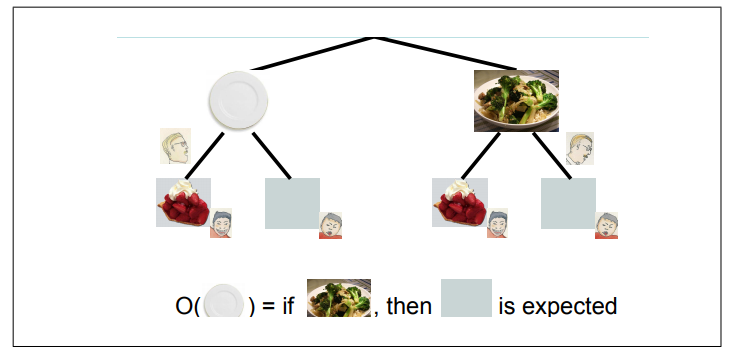
\includegraphics[scale=0.8]{2.png}
    \caption{Expectation, from [van der Torre, 2010]}
    \label{fig:my_label}
\end{figure}
\end{center}

You can also model this example as a game tree. In the first two branches the son can decide whether he eats his vegetables or not. Therefore the son has a model of how the parents will react to his behavior. He takes the response of his parents into account to make his decision.\\
In deontic logic you would propose, based on a violation game, it is obligatory to eat his vegetables and when the son does not then he expects that not eating his vegetables leads to a violation. (illustrated in Fig. 2)\\
Here we could express this as a logical term:\\
$O(eatVegetables) = notEatingVegetables \to noDessert$. \\

The general definition of obligation based on violation games extends this basic idea to behavior over periods of time, for example van der Torre suggests to separate the behavior into different phases.\\
You can say that it is obligatory to eat vegetables. Not eating the vegetables is a strategy that leads to violation. This is what van der Torre calls an equilibrium.\\
When you try to separate the behavior into different phases you can say that in the first phase the son eats his vegetables and the violation does not occur. In the game tree this violation can occur but only implicit since this is no situation you can reach in our dinner problem.\\
The second phase describes that not eating the vegetables is identified with the absence of dessert.\\
The third phase is the most interesting. The son can decide to eat or not to eat his vegetables. As long as the norm is in force he will believe to be sanctioned when he does not eat his vegetables. When the sanction is not applied most of the time you have reached a fourth phase where you can say that the norm is no longer on force. (illustrated in Fig. 3)\\

We can express this equilibrium as:\\
$O(eatVegetables) = notEatingVegetables$ with $noDessert$\\
So the absence of dessert is not implied, it is combined with the fact not eating the vegetables and this is equal to the obligation to eat your vegetables.\\
\begin{center}
\begin{figure}[!htb]
    \centering
    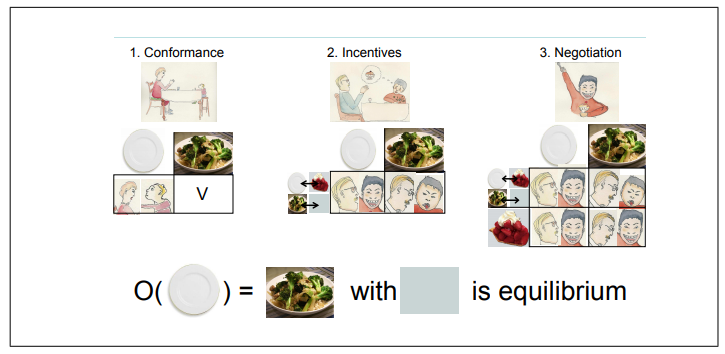
\includegraphics[scale=0.8]{3.png}
    \caption{Expectation, from [van der Torre, 2010]}
    \label{fig:my_label}
\end{figure}
\end{center}

Based on these considerations van der Torre made the following Definitions.\\
\begin{definition}
Violation games are social interactions
among agents to determine whether violations have occurred, and which sanctions
will be imposed for such violations. A normative system is a specification of violation
games.\cite{b2}\\
\end{definition}

If we consider the hijacked-plane-example we can say that the terrorist who hijacked a plane is playing a violation game. A game of life and death not only with the people in the plane and in the skyscraper but in particular with the people who may shoot down the plane. The terrorist takes into account that he gets shot like the son takes into account not getting a dessert.\\
Since norms don't have truth values you cannot easily say that two normative systems are logically equivalent. Taking equivalence of normative systems is a fundamental principle of deontic logic. Also you can say that a norm is accepted by a normative system  if adding it to the normative system leads to an equivalent normative system. Also you can say that a norm is redundant in a normative system if removing it from the normative system leads to an equivalent normative system.\\

\begin{definition}
Two normative systems are equivalent if and only if they define the same set of violation games.\cite{b2}\\
\end{definition}

Also van der Torre now gives a more precise definition of an autonomous system.

\begin{definition}
A system is autonomous if and only if it can play violation games.\cite{b2}\\
\end{definition}


\section{Norm creation games}
We explained how norms can be used as a description of violation games. So violation games are the basis of normative reasoning and deontic logic. But more complex games must be considered too for example norm creation games, van der Torre will later define this term.\\
Van der Torre considers the following example: A child is in the water and there is one bystander. There are good chances that the bystander will jump into the water and save the child. But if you imagine 100 bystanders the child will probably drown because no one would feel obligated to jump into the water.\\
So now you can consider norm creation games as an extension of violation games. You could create a norm where everyone has the norm for himself to jump into the water so the child will not drown.\\
So this is what people refer as a mental modality, it defines the assumptions different agents have about each other in a social context. For this case the mental modality of every bystander is to jump into the water or else the child will drown.\\
So a more general definition of a normative system is the following.\\

\begin{definition}
Norm creation games are social
interactions among agents to determine which norms are in force, whether norm violations have occurred, and which sanctions will be imposed for such violations. A
normative system is a specification of norm creation games.\cite{b2}\\
\end{definition}

You can even more specify this when you discriminate among the people. For example if you assume that not every person is obligated to jump into the water e.g just the good swimmers or tall people and so on. There more you know about the situation the more you can say about the protocol that leads to the norm.\\
Van der Torre says that one can derive obligations from norms and that the protocols for norm creation must be represented to model more complex games. So this are the semantics for the new deontic logic based on violation games.
\section{Conclusion}
To sum up this ideas we can say that time, actions, mental modalities and permissions are important for violation games. Also you get an understanding of the idea of violations conditions which do not necessarily lead to sanctions. Violation games can be considered as a metaphor to bring these problems together and study their interdependencies. \\
As far as we understand we cannot use the approach of violation games in every scenario. If we again consider our hijacked-plane example: You cannot really negotiate with the terrorist or give him incentives. But the idea of a norm creation game is a possible approach to model this problem. For instance we could create a new norm that everyone is obligated to save as many lives as possible. But even here we cannot really guarantee that this norm will be in force the whole time as long as some individuals have their own norm they will act to.\\
So in our opinion it is kind of impossible to model every moral dilemma and come to a conclusion. The best way to handle this is to model the behavior between the actors which are in charge to make a decision in this matter. We could create new norms for the special case of a hijacked plane (e.g save as many lives as possible) or start negotiations between the actors in charge to make the best out of the situation according to the norms that have been violated so at least the actors are trying prevent more violations of norms.\\

But one question remains: How can deontic logic be based on both norm and detachment, as well as decision and game theory?\\
Even the approach of decision and game theory is very complex and cannot easily be applied on specific situations like we pointed out in the section above.\\
If we try to combine the detachment approach with our hijacked plane example we could argue that it is possible to detach the obligation to save as many lives as possible in this specific situation.\\
But we cannot to this without any consequences because if we detach a norm we would probably change the whole violation game or even create a paradox due to some norms that were created in a norm creation game before. Also violation games depend on several aspects like mental modalities as said before. So if a mental modality forbids the actors the detach a norm we just simply cannot combine the detachment approach with our hijacked plane example.
Surely we can find situations where we can start to combine these two approaches but the more agents are involved in the normative systems the harder it gets to adhere to the norms we created.
\begin{thebibliography}{00}

\bibitem{b1} https://en.wikipedia.org/wiki/Social\_norm
\bibitem{b2} L. van der Torre. Violation games: a new foundation for deontic logic. Journal of
Applied Non-Classical Logics, 20(4):457–477, 2010.
\bibitem{b3} Gabriella Pigozzi, Leendert van der Torre. Multiagent Deontic Logic
and its Challenges
from a Normative Systems Perspective
\end{thebibliography}
\vspace{12pt}


\end{document}
